\documentclass[11pt]{article}
\usepackage{graphicx}
\usepackage{tcolorbox}
\usepackage{listings}
\usepackage{physics}
\usepackage{caption}
\usepackage{subcaption}
\usepackage{geometry}
\usepackage{float}
\usepackage{url}
\usepackage{braket}
\usepackage{amsfonts}
\usepackage{amsbsy}
\usepackage{tikz}
\usetikzlibrary{quantikz2}

\usepackage[colorlinks=true,citecolor=blue, linkcolor=black]{hyperref}

\usepackage[T1]{fontenc}
\usepackage{fontspec}
\setmainfont{Georgia}

\usepackage{biblatex}
\addbibresource{references.bib} 


\interfootnotelinepenalty=10000

\lstset{
  basicstyle=\ttfamily,    
  breaklines=true, 
  keywordstyle=\color{blue}, 
}

\setlength\parindent{0cm}
\setlength{\parskip}{11pt}
\geometry{portrait, margin=1in}

\title{
    \vspace{-2.5cm}
    Quantum Computing Final Project
}
\author{
    Samuil Donchev, William Galvin
}
\date{
    \vspace{-.75cm}
    December 2023
}

\begin{document}

\maketitle

\begin{abstract}
Solving the electron structure problem is of great interest in quantum chemistry. One approach for this task, the Ritz variational method, is to construct a molecular Hamiltonian and minimize its expected value over a trial wave function. On quantum computers, this approach promises to one day outperform state-of-the-art classical techniques. In this paper, we explore the Ritz method from end-to-end, discussing the construction of the molecular Hamiltonian, the selection and parameterization of a trial function, and and the optimization of the system. Finally, we demonstrate this approach on several small molecules following a tutorial from PennyLane, and present our own matrix algebra-based simulation framework.
\end{abstract}

\section{Introduction}
In the following pages, we will summarize how the Variational Quantum Eigensolver (VQE) can be applied to approximate the ground state of a molecule. A molecule is a group of atoms bonded together. Every atom has electrons that occupy orbitals, with each atom having a varying number of orbitals of different energy levels. These orbitals change when several atoms bond together to form a molecule. Such orbitals are called molecular orbitals. Each molecular orbital contains two spin orbitals, one for the spin-up electron and the other for the spin-down electron. The ground state of an electron is simply the electron configuration in which the electrons occupy the lowest energy orbitals. 

The VQE technique allows us to approximate the lowest energy state of the molecule using the Molecular Hamiltonian $H$ and the molecule's wave function $\Psi$. We will explain in detail what the Hamiltonian and wave function represent, how they are encoded in a quantum computer, and how they can be used to calculate the ground state energy of a molecule. 

\section{The Molecular Hamiltonian}
The Hamiltonian is a unary operator, $H$, that evaluates to the total energy of a system. The set of values that $H$ can take is called the system’s \emph{spectrum}---however, it is often more useful to consider the expected (“average”) value of a Hamiltonian, as physical experimental measurements are averages \cite{Skylaris-L2}.

A \emph{molecular} Hamiltonian describes the energy of a molecule, and is composed of terms describing 1) the kinetic energy of each charged particle in the molecule---protons in the nuclei and electrons---and 2) the potential energy from interactions between particles. Coulomb’s Law states that like forces repel and opposite forces attract. This means that a molecular Hamiltonian will have repulsion terms for each electron-electron and nucleus-nucleus pair, and attraction terms for each election-nucleus pair \cite{Skylaris-L2}. In essence, the energy of a molecule is determined by interactions between charged particles.

To reduce the number of terms in $H$, the Born-Oppenheimer approximation sets the kinetic energy terms of nuclei to $0$, since nuclei move much slower than electrons. This does not change the number of interaction terms with electrons, though nucleus-nucleus terms are sometimes also omitted (with neither nucleus moving, any nucleus-nucleus term is constant with respect to electron configurations). Such a formulation is called the electronic Hamiltonian, $H_e$, also known as the ``clamped nucleus Hamiltonian" \cite{Skylaris-L2}.

\subsection{Molecular Hamiltonians in Quantum Computing}
Our first formula for $H_e$ follows naturally from the definition above, and is given by 
$$
H_e =
\sum_{i=1}^{N} \left( -\frac{1}{2} \nabla_{x_i}^2 \right) +
\sum_{i=1}^{N} \sum_{j < i} \frac{1}{|x_i - x_j|} -
\sum_{i=1}^{N} \sum_{I = 1}^{M} \frac{Z_I}{|x_i - R_I|}
$$
In this notation, there are $N$ electrons and $M$ nuclei, with $x_i$ denoting the $i$-th electron and $R_I$ denoting the $I$-th nucleus; the $Z_I$ term is the number of protons in the $I$-th nucleus. In the leftmost term, we have the Laplacian ($\nabla^2$) operator, which gives the kinetic energy for each electron. (Notice that in the $H_e$ approximation, there is no kinetic energy term for the nuclei.) In the center term, we have the electron-electron repulsion terms, which lead to higher potential energy when electrons are close. Finally, the rightmost term describes the electron-nucleus attraction forces, which lead to higher potential energy when electrons and nuclei are far apart \cite{Baidu}.

An important term in $H_e$ is the one representing the electron-electron interactions, $\sum_{i=1}^{N} \sum_{I = 1}^{M} \frac{Z_I}{|x_i - R_I|}$. This term is actually very difficult to compute as we do not know the pairwise distances between every electron pair. Thus, we can apply the Hartree-Fock Approximation, which states that we can approximate the electron-electron repulsion forces as the force each electron feels due to the mean electronic field \cite{Ivo}. This is usually calculated iteratively and may not always converge. 

While this formulation follows directly from our initial formulation, it quickly becomes cumbersome with large systems. 

An alternative representation of a Hamiltonian is known as the ``second quantization formalism" or ``occupation number basis" representation. In this encoding, we consider wave functions and spin-orbitals. A wave function relates the state of a particle system to an amplitude, which can be interpreted as the probability of the particle being found in that state. A spin orbital is a molecular orbital described by both spatial coordinates and spin; in a particular spatial region, there can be at most one electron with each spin (up or down). We can describe the likelihood of an electron being in a spin orbital using a wave function \cite{Skylaris-L4}.

With $S$ spin orbitals\footnote{Figuring out exactly how many spin orbitals a molecule has is non-trivial, but involves considering the orbitals of a molecule's constituent atoms and the ways in which electrons are shared in chemical bonds}, occupation number representation takes the form $\ket{n_0, n_1, \dots, n_{S-1}}$ where each $n_i$ is either $0$ or $1$, representing the absence or presence of an electron in the $i$-th spin orbital. The Hamming weight (number of $1$s) is the total number of electrons and determined by the molecule itself---all that’s left to find is the probability of the different states \cite{Oslo, Givens}.

In this form, there are two important new operators: electron creation, $c^{\dagger}$, and electron annihilation, $c$. $c_i^{\dagger}$  creates an electron in the $i$-th orbital and $c_i$ destroys an electron in the $i$-th orbital. These can be written as 
$$
\begin{array}{lcl}
    c^{\dagger}_i &=& \displaystyle Z \otimes Z \otimes \dots \otimes Z \otimes \left[\frac{X - iY}{2} \right] \otimes I \otimes I \otimes \dots \otimes I \\\\

    c_i &=& \displaystyle Z \otimes Z \otimes \dots \otimes Z \otimes \left[\frac{X + iY}{2} \right] \otimes I \otimes I \otimes \dots \otimes I
\end{array}
$$
Where each of the $S$ spin orbitals has a corresponding $\mathbf{C}^{2 \times 2}$ matrix; when these are combined via tensor product, they create a $\mathbf{C}^{2^S \times 2^S}$ matrix. For the indices less than $i$, the matrix is the Pauli-$Z$ matrix $\sigma_z = \left[\begin{array}{cc}
   1  &  0 \\
   0  &  -1
\end{array} \right]$; the $i$-th matrix is $\displaystyle \left[\frac{X \mp iY}{2} \right]$ where $\sigma_x = \left[\begin{array}{cc}
   0  &  1 \\
   1  &  0
\end{array} \right],  \:\:
\sigma_y = \left[\begin{array}{cc}
   0  &  -i \\
   i  &  0
\end{array} \right]$; and for indices greater than $i$, the identity matrix is used \cite{Whitfield_2011}.

How does this relate to the electronic Hamiltonian? It turns out that any Hamiltonian can be written as a combination of \emph{electron creation-electron annihilation} products, since as long as creation and annihilation come as a pair, the total number of particles is respected. The electron-nucleus attraction term (``one-electron operator") and the electron-electron repulsion term (``two-electron operator") can each be expressed in terms of creation and annihilation operations, then combined to form $H_e$. This means that we can represent our Hamiltonian---the energy operator---in terms of $\ket{n_0, n_1, \dots, n_{S-1}}$ \cite{Gusmao}.

In fact, the Hamiltonian (with Born-Oppenheimer approximation) can be written as the weighted sum of products of creation and annihilation operators \cite{Rongxin}:
$$
H_e = 
\sum_{p,q} h_{pq} c^{\dagger}_{p} c_{q} + 
\frac{1}{2} \sum_{p,q,r,s} h_{pqrs} c^{\dagger}_p c^{\dagger}_q c_r c_s
$$
Here, $\{p, q, r, s \}$ are indices into spin orbitals; the weights $h$ are determined by the Coulomb attraction/repulsion laws; and the first term is one-electron, the second term is two-electron.

We can see that for a system with $S$ spin orbitals and thus $q$ qubits, $H_e \in \mathbf{C}^{2^q\times 2^q}$. Since this quickly becomes extremely large, there is one final transformation to make so that our Hamiltonians can act as quantum gates: expressing them as a linear combination of the tensor product of Pauli matrices \cite{Delgado-Hamiltonians}. Pauli matrices---the same ones that we expressed $c^{\dagger}_i$ and $c_i$ in---are the set of complex  $2 \times 2$ matrices that are Hermitian, unitary, and involutory (inverse of itself):
$$
\sigma_x = \left[\begin{array}{cc}
   0  &  1 \\
   1  &  0
\end{array} \right],  \:\:
\sigma_y = \left[\begin{array}{cc}
   0  &  -i \\
   i  &  0
\end{array} \right], \:\:
\sigma_z = \left[\begin{array}{cc}
   1  &  0 \\
   0  &  -1
\end{array} \right]
$$
The Pauli matrices and the identity, $I$, form a basis for the vector space of all Hermitian matrices, and as a result, all $H_e$.

When we make this transformation such that $H_e = \sum_j C_j \otimes_i \sigma_i^{(j)}$ (for some $C_j \in \mathbf{R}, \sigma \leftarrow $ tensor product of Pauli matrices), we no longer have to need a single, giant gate and can effectively consider $H_e$ as smaller gates that act on individual pairs of qubits. After finding the coefficients of the Pauli matrices that combine to form the Hamiltonian, $H_e$ can be evaluated from these coefficients \cite{Rongxin}. 

\section{The Variational Method}
Consider $\Psi_0$ as the wave function describing the exact ground state of a molecule, and $E_0$ to be the corresponding energy. Schrödinger's equation tells us that $H\Psi_0 = E_0\Psi_0$. Now consider $\psi$ as some trial wave function, and $\frac{\braket{\psi|H|\psi}}{\braket{\psi|\psi}}$ to be the expected value of the Hamiltonian with respect to this $\psi$ state, which also happens to be the lowest eigenvalue of $H_e$. Here, the expected value is guaranteed to provide an upper bound for $E_0$ \cite{Berekely}. 

If $\psi$ is some function of $\theta$, then this upper bound will vary with $\theta$. To find the lowest upper bound according to the the trial function, we can take the gradient of the expectation with respect to $\theta$ and set it equal to $0$, thereby finding the minima. In this setup, all of the typical optimization tools become available to us \cite{Berekely}.

In general, any $\psi$ may be chosen where $\frac{\braket{\psi|H|\psi}}{\braket{\psi|\psi}}$ can be calculated\footnotemark{} \cite{Berekely}, but good trial functions typically 1) have wave function-like characteristics (continuous, single-valued, etc) 2) have a similar shape to the true wave function $\Psi_0$ and 3) have the same asymptotic behavior and/or boundary conditions as the true function $\Psi_0$ \cite{LibreChem}. As a result, trial functions are often ``guessed" from domain knowledge of related problems---one such family of ``guesses" can be constructed from a series of Givens rotations.

\footnotetext{To calculated this expected value, let $\psi^{*}$ be the complex-conjugate of $\psi$ and $\int \cdot \: d\tau$ be the integral over all space; then,  $\frac{\braket{\psi|H|\psi}}{\braket{\psi|\psi}} = \frac{\int\psi^{*}H\psi d\tau}{\int \psi^{*}\psi d\tau}$ \cite{Cresser}. More concretely, evaluate $H\psi$ as ``the total energy of the wave function'', multiply this value with the complex-conjugate of the wave function and integrate over space, and divide by the integral of the wave function with its complex-conjugate, which acts as a normalizing term. If we think of $\psi$ as a vector where $\psi_i \in \mathbf{C}$ describes the amplitude (relative probability) of observing the $i$-th state, the complex-conjugate $\psi^*$ is simply the element-wise complex-conjugate of the vector.}

\subsection{Givens Rotations for Electronic Excitations}
Recall that in occupation number representation, a state takes the form $\ket{n_0, n_1, \dots, n_{S-1}}$ with $n_i \in \{0, 1 \}$. In the Hartree-Fock ground state, electrons fill the lowest available orbitals: $\ket{1, 1, \dots, 0, 0}$ \cite{Oslo, Givens}. An \emph{excitation} occurs when an electron moves from a lower orbital to a higher, previously unoccupied orbital. 

For example, the Hartree-Fock ground state of a two-orbital, one-electron system is $\ket{1, 0}$ and can be excited to the state $\ket{0, 1}$. We can represent this two-orbital system with two-qubits, which can be observed in the states $\ket{\{0,1\}^2} = \ket{00}, \ket{10}, \ket{01}, \ket{11}$. As a wave function we can represent our original HF ground state as 
$$\psi_{\ket{1, 0}} = 
0\ket{00} + 1\ket{10} +  0\ket{01} + 0\ket{11} = \left[\begin{array}{cccc}
 0 & 1 & 0 & 0
\end{array}\right]
$$
We can similarly represent our excited state as 
$$\psi_{\ket{0, 1}} = 
0\ket{00} + 0\ket{10} +  1\ket{01} + 0\ket{11} = \left[\begin{array}{cccc}
 0 & 0 & 1 & 0
\end{array}\right]
$$
From this, it becomes clear that an excitation is a transfer of wave function amplitude between the ground state and the excited state. In this context, we can represent excitations as \emph{state-transition matrices}.\footnote{For a state-transition matrix $A$, $A_{ij}$ gives the probability of moving from state $i$ to state $j$. If we have some row vector $\mathbf{v}^t$ where $\mathbf{v}_i^t$ is the probability of observing state $i$ after $t$ transitions, we can find $\mathbf{v}^{t+1} = \mathbf{v}^{t}A$.}

This is the foundation from which \emph{Givens rotations} build. A Givens rotation parameterized by $\theta$, $G(\theta)$, describes the probability of a particular excitation occurring. For an excitation from orbital $i$ to orbital $j$, a Givens rotations maps a ``swap" in probability between all pairs of states $\ket{n_0, n_1, \dots n_{i-1}, 1, \dots, n_{j-1}, 0, \dots}$ and  $\ket{n_0, n_1, \dots n_{i-1}, 0, \dots, n_{j-1}, 1, \dots}$. 

As a state-transition matrix $G$, this takes the form of the identity matrix, $I$, with the exception that if $a$ is the index of a state from which the excitation can occur and $b$ is the index of the corresponding excited state, then 
$$
\begin{array}{rcr}
     G_{aa} &=& \cos(\theta/2) \\
     G_{ab} &=& -\sin(\theta/2) \\
     G_{ba} &=& \sin(\theta/2) \\
     G_{bb} &=& \cos(\theta/2)
\end{array}
$$ 
From our earlier example, there is exactly one pair of states in which the excitation can occur, and we can write the Givens rotation matrix as 
$$
G = \left[\begin{array}{cccc}
   1 & 0 & 0 & 0 \\
   0 & \cos(\theta/2) & -\sin(\theta/2) & 0 \\
   0 & \sin(\theta/2) & \cos(\theta/2) & 0 \\
   0 & 0 & 0 & 1
\end{array}
\right]
$$
After applying this rotation matrix to our original state, we have $
\left[\begin{array}{cccc}
    0 & \cos(\theta/2) & -\sin(\theta/2) & 0
\end{array}
\right]
$. If we pick $\theta = \pi$, this gives us the same formulation as our original excitation; since we're working with qubits, the probability of each state is given by the square of the amplitude, and $(-\sin(\pi/2))^2 = 1$. We can also see that if we pick some other $\theta$, we can create a superposition of states whose relative probabilities are a function of $\theta$.

Consider a similar excitation, but in a three-orbital system. Now there are $2^3 = 8$ total states for our wave function, and two pairs of states in which an electron from the first orbital can be excited into the second: $\ket{100} \to \ket{010}$ and $\ket{101} \to \ket{011}$. Thus our Givens rotation for this excitation would take the form 
$$ G = 
\left[\begin{array}{cccccccc}
1 & 0 & 0 & 0 & 0 & 0 & 0 & 0 \\
0 & \cos(\theta/2) & -\sin(\theta/2) & 0 & 0 & 0 & 0 & 0 \\
0 & \sin(\theta/2) & \cos(\theta/2) & 0 & 0 & 0 & 0 & 0 \\
0 & 0 & 0 & 1 & 0 & 0 & 0 & 0 \\
0 & 0 & 0 & 0 & 1 & 0 & 0 & 0 \\
0 & 0 & 0 & 0 & 0 & \cos(\theta/2) & -\sin(\theta/2) & 0 \\
0 & 0 & 0 & 0 & 0 & \sin(\theta/2) & \cos(\theta/2) & 0 \\
0 & 0 & 0 & 0 & 0 & 0 & 0 & 1 \\
\end{array} \right]
$$

So far we have considered \emph{single excitations}, in which a single electron moves between orbitals. We can also consider \emph{double excitations}, in which a pair of electrons move together. For example, $\ket{1100} \to \ket{0011}$ or $\ket{010100} \to \ket{000011}$. The Givens rotation matrix is constructed in the same fashion, by finding pairs of states that correspond to valid realizations of the excitation.

In a $q$-qubit system, the number of pairs of states affected by an excitation of $n$ electrons is given by $2^{2^{q} - 2n}$; i.e., for each of the qubits representing an orbital not involved in the excitation, double the number of pairs to consider. 

In general, a particular excitation can be represented with $G \in \mathbf{C}^{2^q \times 2^q}$, a unitary matrix that maps between pairs of states $(a, b)$ with  
$$
\begin{array}{rcr}
     G_{aa} &=& x \\
     G_{ab} &=& y \\
     G_{ba} &=& z \\
     G_{bb} &=& w
\end{array}
$$
where $|x|^2 + |y|^2 = |z|^2 + |w|^2 = 1$ and $xy^* + wz^* = 0$ to ensure unitarity \cite{Arrazola_2022}. Choosing to use this particular $\sin$-$\cos$ formulation is an example of ``guessing" an appropriate wave function. 

As a circuit, a Givens single rotation can be expressed as
$$
\begin{quantikz}
&\ctrl{1}&\gate{\theta/2}&\targ{}&\gate{-\theta/2}&\targ{}&\ctrl{1}& \\
&\targ{}&&\ctrl{-1}&&\ctrl{-1}&\targ{}&
\end{quantikz} 
$$
where the rotation gates are Pauli-Y rotations. Double excitations can similarly be expressed in terms of Pauli-Y rotations, Hadamard gates, and CNOT gates \cite{Quantum}.

To construct our wave function from these Givens rotations, we begin with our HF ground state
$$
\psi_{\text{HF-ground}} = \ket{11\dots 00}
$$
We then consider each possible single- and double-excitation, a set which depends on the number of orbitals and electrons in our system, and their associated Givens rotations $G_i$ each parameterized by an independent $\theta_i$. Since these are state-transition matrices, we find our final state as 
$$
\psi(\boldsymbol{\theta}) = \psi_{\text{HF-ground}} \prod_{i} G_i(\theta_i)
$$
 
\section{Optimization}
Once we have constructed some trial wave function $\psi$ with parameters $[\theta_0,\theta_1, \dots, \theta_n]$ and calculated the molecular Hamiltonian $H$, we need to minimize the expected value of the Hamiltonian. 
\begin{enumerate}
    \item \textbf{Define cost function.} Here the cost is the expected value of the Hamiltonian with respect to the wave function.
    \item \textbf{Initialize wave function parameter values.} Common choices are either 1) all zeros or 2) uniformly random between $0$ and $2\pi$.
    \item \textbf{Perform gradient descent}. To find the gradient of the cost function with respect to the wave function parameters, we need to be able to differentiate Givens rotations. These are composed from Pauli-Y rotations, and $\frac{d}{d\theta}f(R_y(\theta)) = 12[f(R_y(\theta + \pi/2)) - f(R_y(\theta-\pi/2))]$ where $f$
 is an expectation value depending on $R_y(\theta)$. \cite{Quantum}.
    \item \textbf{Update parameters} according to $\theta = \theta - \alpha \nabla f$.
    \item \textbf{Repeat} 3-4 until maximum iterations or values converge within a specified tolerance.
    \item \textbf{Use converged parameters} to determine wave function and find the probability of electrons in each permissible state.
\end{enumerate}
Once we have the best approximation of the wave function, we can use it along with the Hamiltonian to calculate the approximated ground state energy of the molecule.

\section{Results}
We apply this routine to four small molecules: H$_2$, H$_4$, OH$^-$, and H$_2$O. In doing so, we confirm that both the wall-clock-time required for the simulation  and the number of learnable parameters grow exponentially with respect to the number of qubits (see table below). We also find that most individual excitations are  quite unlikely; in the figure below, we plot histograms of $\sin(\theta_i)^2$, which can be interpreted as the probability of excitation $i$ occurring.
\begin{figure}[!h]
  \begin{minipage}[t]{.6\linewidth}
    \centering
    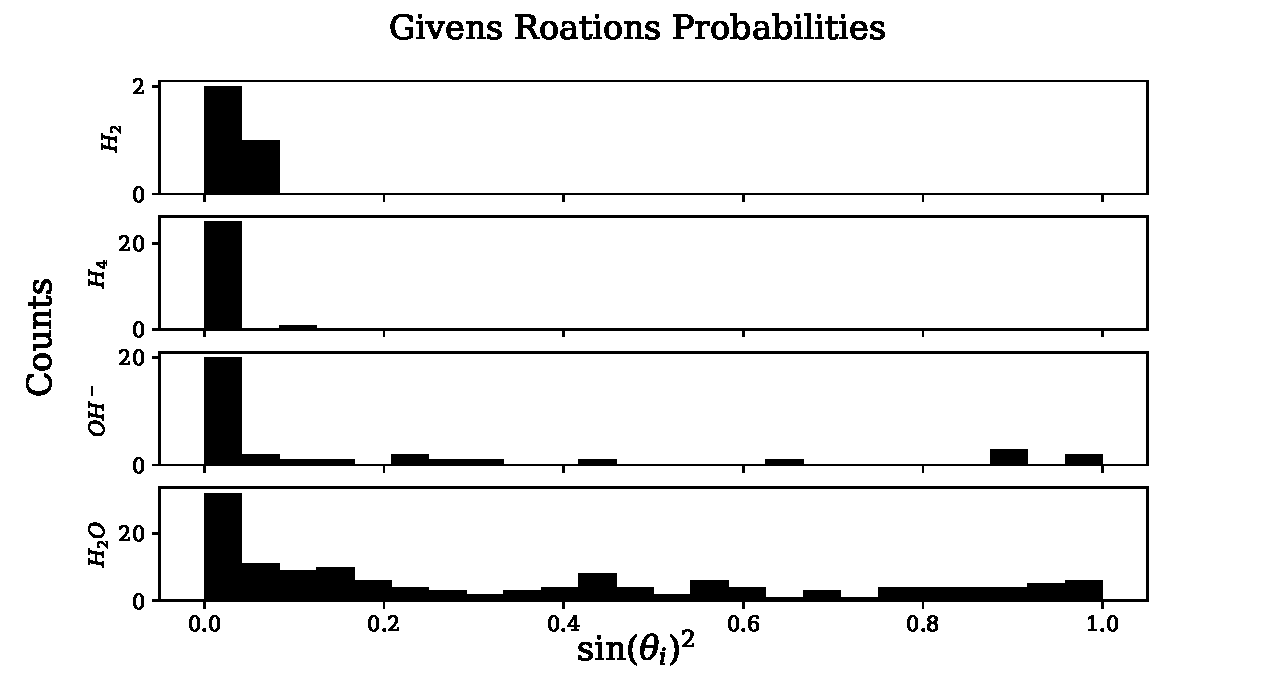
\includegraphics[scale=0.45]{images/results.pdf}
  \end{minipage}\hfill
  \begin{minipage}[t]{.4\linewidth}
  \centering
  \vspace{-4.525cm}
  \renewcommand{\arraystretch}{1.65}
    \begin{tabular}{|c|c|c|c|} \hline 
         \textbf{Molecule}&  \textbf{Qubits}&  \textbf{dim}$(\theta)$& \textbf{Time} \\ \hline 
         H$_2$&  4&  3& 43 s\\ \hline 
         H$_4$&  8&  26& 1 m\\ \hline 
         OH$^-$&  12&  35& 24 m\\ \hline
         H$_2$O&  14&  140& 48 m\\ \hline
    \end{tabular}
    \renewcommand{\arraystretch}{1}
  \end{minipage}
\end{figure}


\section{Time Complexity}
We will quickly explore the time complexity for each step of the VQE. For a more complete explanation, see \cite{complex}.

The Hamiltonian matrix construction takes $\mathcal{O}(n^4)$ where $n$ is a basis function, which accounts for the Hamiltonian terms. From there, encoding the Hamiltonian into the Jordan-Wigner form takes $\mathcal{O}(n)$, where $n$ is the number of qubits. These steps aren't what usually contribute to the main computational struggle, though. What determines the time complexity is the wave-function estimation and achieving the desired precision of our answer. PennyLane uses the k-UpCCGSD ansatz method of setting up the wave-function using the single and double excitation given rotations previously mentioned. The time complexity is $\mathcal{O}(kn)$ where $k$ is the number of thetas and $n$ is the number of single and double excitation terms in the quantum circuit. Measuring each register also takes $\mathcal{O}(n)$ time, thus the total complexity for this step is $\mathcal{O}(kn^2)$. The last step is optimizing the $\theta$s to determine the ground state energy of the Hamiltonian. In the Pennylane tutorial, we stopped optimizing until we reached a certain precision threshold $\epsilon$ or 100 iterations. This would make our runtime $\mathcal{O}(1)$ as the 100 iterations are constant. In practice though, optimization ends once the precision threshold is met. Thus, for a precision of $\epsilon$ the time complexity to calculate each theta is $\mathcal{O}(\frac{1}{\epsilon^2})$. Thus the total time complexity to approximate the wave function and optimize for the thetas is $\mathcal{O}(\frac{kn^2}{\epsilon^2})$ \cite{complex}.

\section{Code}
The code for this project is available here: \texttt{\href{https://github.com/william-galvin/DD2367-Quantum-Chemistry}{https://github.com/william-galvin/DD2367-Quantum-Chemistry}}. In this repository we present two modules:
    \subsection{\texttt{pennylane/}} A copy of the PennyLane VQE tutorial \cite{Delgado-VQE} with slight modifications to allow for larger molecules. This is the program used to generate data for our results section (above).
    \subsection{\texttt{vcvqe/}} The ``Very Classical Variational Quantum Eigensolver"---this program is an end-to-end implementation of most of the concepts discussed in this paper, without a dependency on PennyLane or any other quantum computing framework. 

    Rather, we use \texttt{numpy} \cite{numpy}, \texttt{JAX} \cite{JAX}, and \texttt{PySCF} \cite{PySCF} to create a matrix algebra-based implementation of the molecular Hamiltonian and Givens rotations, as well as to perform a simple optimization routine. \texttt{PySCF} is used to calculate the one- and two-electron Coulomb integrals ($h_{pq}$ and $h_{pqrs}$), and \texttt{JAX} is used to automatically differentiate the expected value of the Hamiltonian with respect to $\theta$ parameters, allowing for an extremely simple gradient descent-based optimization routine. 

    Of course, this approach is problematic. Storing and manipulating the state vector and Hamiltonian for even a small molecule quickly becomes prohibitive in memory. For example, a water molecule requires 14 qubits and therefore a Hamiltonian with $2^{14} \times 2^{14}$ entries. Using 64-bit complex numbers, this would be more than 2 GB. As a result, the VCVQE is only practical with small molecules, like H$_2$ and H$_4$.

    Furthermore, the energies calculated by this approach account for only electron-electron and electron-nucleus interactions and electron kinetic energy, under the Born-Oppenheimer and Hartree-Fock approximations. It does not incorporate nucleus-nucleus interactions, nuclear kinetic energies, or pairwise electron-electron energies. As such, the energies calculated here do not match the energies calculated by PySCF and PennyLane.

    Nonetheless, the construction of the electronic Hamiltonian (\texttt{/vcvqe/hamiltonian.py}) and the formulation of the trial wave function (\texttt{/vcvqe/givens.py}) provide an instructive and intuitive view into the Ritz variational method and the VQE.


\newpage
\printbibliography 


\end{document}
